\documentclass[12pt]{article}
\usepackage{amsmath,amssymb,amsfonts}
\usepackage{tikz}

\begin{document}

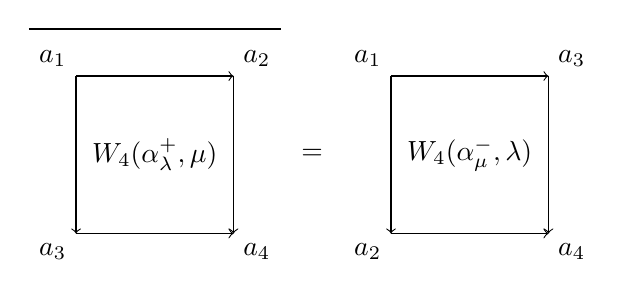
\begin{tikzpicture}[scale=2]
\draw [-to](1,1)--(2,1);
\draw [-to](1,2)--(2,2);
\draw [-to](1,2)--(1,1);
\draw [-to](2,2)--(2,1);
\draw [thick] (0.7,2.3)--(2.3,2.3);
\draw (1,1)node[below left]{$a_3$};
\draw (1,2)node[above left]{$a_1$};
\draw (2,1)node[below right]{$a_4$};
\draw (2,2)node[above right]{$a_2$};
\draw (1.5,1.5)node{$W_4(\alpha_\lambda^+,\mu)$};
\draw (2.5,1.5)node{$=$};
\draw (3.5,1.5)node{$W_4(\alpha_\mu^-,\lambda)$};
\draw [-to](3,1)--(4,1);
\draw [-to](3,2)--(4,2);
\draw [-to](3,2)--(3,1);
\draw [-to](4,2)--(4,1);
\draw (3,1)node[below left]{$a_2$};
\draw (3,2)node[above left]{$a_1$};
\draw (4,1)node[below right]{$a_4$};
\draw (4,2)node[above right]{$a_3$};
\end{tikzpicture}

\end{document}